%%%%%%%%%%%%%%%%%%%%%%% file template.tex %%%%%%%%%%%%%%%%%%%%%%%%%
%
% This is a general template file for the LaTeX package SVJour3
% for Springer journals.          Springer Heidelberg 2010/09/16
%
% Copy it to a new file with a new name and use it as the basis
% for your article. Delete % signs as needed.
%
% This template includes a few options for different layouts and
% content for various journals. Please consult a previous issue of
% your journal as needed.
%
%%%%%%%%%%%%%%%%%%%%%%%%%%%%%%%%%%%%%%%%%%%%%%%%%%%%%%%%%%%%%%%%%%%
%
% First comes an example EPS file -- just ignore it and
% proceed on the \documentclass line
% your LaTeX will extract the file if required
\begin{filecontents*}{example.eps}
%!PS-Adobe-3.0 EPSF-3.0
%%BoundingBox: 19 19 221 221
%%CreationDate: Mon Sep 29 1997
%%Creator: programmed by hand (JK)
%%EndComments
gsave
newpath
  20 20 moveto
  20 220 lineto
  220 220 lineto
  220 20 lineto
closepath
2 setlinewidth
gsave
  .4 setgray fill
grestore
stroke
grestore
\end{filecontents*}
%
\RequirePackage{fix-cm}
%
\documentclass{svjour3}                     % onecolumn (standard format)
%\documentclass[smallcondensed]{svjour3}     % onecolumn (ditto)
% \documentclass[smallextended]{svjour3}       % onecolumn (second format)
%\documentclass[twocolumn]{svjour3}          % twocolumn
%
\smartqed  % flush right qed marks, e.g. at end of proof
%
\usepackage{graphicx}
\usepackage{enumitem}
\usepackage{float}
% \usepackage{caption}
\usepackage{subfig}
\usepackage{cite}
\usepackage{url}
\usepackage{spreadtab}
\usepackage{algorithm,algorithmic}
\usepackage{amsmath}
\usepackage[numbers]{natbib}

\DeclareMathOperator*{\argmin}{argmin} % thin space, limits underneath in displays
\DeclareMathOperator*{\myint}{int} %
%
% \usepackage{mathptmx}      % use Times fonts if available on your TeX system
%
% insert here the call for the packages your document requires
%\usepackage{latexsym}
% etc.
%
% please place your own definitions here and don't use \def but
% \newcommand{}{}
%
% Insert the name of "your journal" with
% \journalname{myjournal}
%
\journalname{}
\begin{document}

\title{Flexible needle and patient tracking using fractional scanning in interventional CT procedures
%\thanks{Grants or other notes
%about the article that should go on the front page should be
%placed here. General acknowledgments should be placed at the end of the article.}
\thanks{Research supported by Kamin grant 57706, Office of the Chief Scientist, Ministry of Trade and Industry, Israel. We thank Eyal Lin and Ronen Shter of GE Healthcare Israel for the CT scans and for their valuable assistance.}% <-this % stops a space
% \thanks{G. Medan and L. Joskowicz are with the CASMIP Laboratory, School of Computer Science and Engineering, The Hebrew University of Jerusalem, Israel (josko@cs.huji.ac.il).}%
}
% \subtitle{Do you have a subtitle?\\ If so, write it here}

\titlerunning{Reduced dose flexible needle and patient tracking}        % if too long for running head

\author{Guy Medan         \and
        Leo Joskowicz %etc.
}

%\authorrunning{Short form of author list} % if too long for running head

\institute{
  L. Joskowicz, G. Medan \at
  CASMIP  Laboratory\\
  School  of  Computer  Science  and  Engineering\\
  The  Hebrew  University of Jerusalem, Israel\\
  \email{josko/gmedan@cs.huji.ac.il}           %  \\
%             \emph{Present address:} of F. Author  %  if needed
}

%\date{Received: date / Accepted: date}
% The correct dates will be entered by the editor
\date{}

\maketitle

\begin{abstract}
We present a new method for flexible needle and patient localization in interventional CT procedures based on fractional CT scanning.
Our method accurately localizes the trajectory of a flexible needle to which a spherical marker is attached at a known distance from the tip with respect to a baseline scan of patient in the CT scanner coordinate frame. 
The localization is achieved with a significantly lower dose compared to a full scan using sparse view angle sampling and without reconstructing the CT image of the repeat scan.
Our method starts by performing rigid registration between the patient and the baseline scan in 3D Radon space computed from the sparse projection data.  It then computes 2D projection difference images in which the flexible needle and the spherical marker appear as prominent features. Their 3D spatial locations are then automatically extracted from the projection images to accurately trace the flexible needle trajectory. To validate our method, we conducted registration and needle trajectory localization experiments in seven abdomen phantom scans using two types of flexible needles. Our experimental results yield a mean needle trajectory localization error of 0.7 $\pm$ 0.2mm and a mean tip localization error of 2.4 $\pm$ 0.9 mm with a x7.5 radiation dose reduction with respect to a full CT scan. The significant radiation dose reduction enables more frequent needle trajectory localization during the needle insertion for a similar total dose, or a reduced total dose for the same localization frequency.
\keywords{
interventional CT \and 
fractional CT scanning \and 
reduced dose CT scanning \and 
flexible needle tracking \and
Radon space registration 
}
\end{abstract}

\section*{Introduction}

Image guided minimally invasive techniques have become commonplace for interventional procedures such as lesion biopsies and aspirations.
In these procedures, a flexible needle is inserted under image guidance towards a target, either manually or using robotic actuators. Repeated imaging is required during insertion to ensure that the needle is advancing in the desired direction and to correct its insertion path as required. Localization errors of a few millimeters in the needle insertion trajectory and its final placement can lead to misdiagnosis, repeated insertion attempts, and failed treatment.

CT guidance is often used in interventional radiology procedures to help the surgeon guide the needle towards the desired target. CT imaging is unique in that it provides real-time high resolution axial in-plane and volumetric images of the patient anatomy and of the needle. However, CT-guided interventions has several limitations and drawbacks. The intervention protocol typically requires the needle to be aligned with the axial plane of imaging as it is being inserted \cite{gupta2014ct}, which in turn requires careful positioning of the patient to allow access to the target.  The presence of the needle in the scanned CT volume introduces imaging artifacts caused by beam hardening and scatter \cite{boas2012ctartifacts}, which can obscure important anatomical structures near the needle tip. Also, the patient's cumulative exposure to ionizing X-ray radiation may increase the risk of cancer \cite{mettler2000ct,chodick2007excess}, which is exacerbated in interventional CT due to frequent, repeated scanning during the procedure.

%Dose reduction for physician
Dose reduction in interventional CT is important both for patients and for the medical staff, since the time spent by physicians, nurses and technologists throughout their careers in the intervention suite necessarily involves exposure to ionizing radiation. While protection equipment is used by medical professionals, the cumulative exposure has been linked to an increased risk of cataracts and cancer \cite{miller2010occupational, sarti2012low}. In interventional CT, it is important to develop methods to prevent excessive dose exposure to the radiologist's hands \cite{stoeckelhuber2005radiation}.

Other imaging modalities used for interventional procedures include ultrasound, X-ray fluoroscopy and cone-beam CT.
Ultrasound is a cost effective imaging solution. However, it only provides 2D cross sectional images with limited resolution and a low signal-to-noise ratio (SNR) \cite{sheafor2000comparison}. Although 3D/4D ultrasound imaging is becoming more available in recent years, its use is still limited in clinical practice.
X-ray fluoroscopy offers improved spatial and intensity resolution, but is not suitable for procedures that require axial views or when complex anatomical relationships must be characterized in 3D during the intervention.
Flat-panel cone-beam CT is a relatively new technology increasingly used in interventional radiology. However it has longer scan times and increased radiation scatter, resulting in increased artifacts compared to multi-detector CT \cite{orth2008cbct}. Recent advances have reduced scan times to 5-20 seconds, with a x2-3 radiation dose reduction \cite{dynact}.

Dose reduction techniques for CT aim to achieve good image quality for a single, standalone scan acquisition. The most common radiation dose reduction technique is tube current modulation, in which the scan is acquired with a lower tube current. However, this technique decreases the scanning signal to noise ratio, which results in noise, lowered imaging contrast and resolution, and introduces imaging artifacts. Several methods have been developed to address these problems, including image denoising \cite{manduca2009projection} and image reconstruction with statistical noise models  \cite{zhang2016statistical,kim2015sparseview,niu2014sparse,liu2014total}. The radiation dose is typically x2-3 that of a full CT scan. 

We have recently introduced a new approach to CT radiation dose reduction in situations in which a full baseline CT scan is available, as is usually the case in interventional CT procedures \cite{medan2017sparse, medan2017reduced}. In our approach, subsequent full dose scanning is replaced by fractional scanning, which consists of the selective acquisition of a sparse set of projection views. Fractional scanning reduces the radiation dose by modulating the current of the X-ray source during its rotation. By exploiting the projection space raw data, registration with the baseline scan and accurate localization of the needle tip in the repeat scans is achieved without reconstruction of the repeat scan image. This technique yields a x9-20 radiation dose reduction. However, this technique is of limited use, as it only tracks the needle tip and assumes that the needle is rigid. It does not take into account the needle bending during the insertion, which frequently occurs in common interventional procedures, e.g., lungs and liver biopsies with thin flexible needles. 

\section*{Previous work}
Various methods have been recently developed to achieve accurate needle insertion with robotic actuators. The proposed methods focus on the mechanical modelling of the robotic system, the patient anatomy, and the needle trajectory planning, with less attention to needle localization from imaging modalities.
Wu et al. \cite{wu2013automatic} and Engh et al. \cite{engh2010percutaneous} describe implementations of a bevel-tip needle steering methods using duty-cycle spinning of the needle that relies on the needle bending tendency due to asymmetry. Such systems model the needle/tissue interaction to execute a control sequence to follow a pre-planned trajectory. Image-based feedback is used as a means to allow corrections of the control sequence mid-insertion by adjusting the planned trajectory based on the actual needle trajectory.
Ben-David et al. \cite{ben2018robotic} describe a robotic system for flexible needle insertion under CT guidance. A dual guiding mechanism consists of a driver unit that advances the needle and a positioning unit that steers the needle during the insertion. A pre-planned 3D trajectory is executed and corrected during the insertion based on full-dose repeat CT scans.
Earlier work by Glozman et al. \cite{glozman2007image} describes robotic flexible needle steering and a needle-tissue mechanical interaction model. The steering feedback is based on 2D in-plane imaging of the needle.

Most works in needle localization from medical images use ultrasound as the imaging modality for localization. Vrooijink et al. \cite{vrooijink2013real} describe a robotics system that positions a 2D ultrasound transducer perpendicular to the needle tip. In this system, needle-induced image artifacts are used to localize the needle tip in the imaged plane. The ultrasound transducer is continuously re-positioned to maintain its orientation relative to the needle tip. An approach combining ultrasound and X-ray imaging is presented in \cite{marinetto2017integration}. In this approach, a free-hand ultrasound probe and a fluoroscopic C-arm are registered using an external optical tracker to produce a fused image in which the needle can be localized and tracked.

Several works describe specific methods to localize the needle trajectory in reconstructed CT images. The authors have developed in previous work a method to 
localize the tip of a straight rigid needle \cite{medan2017reduced}. The needle tip  is computed from 2D projection images in sinogram space. 
Hou et al. \cite{huo2015shape} reconstruct the bevel-tip flexible needle trajectory from full CT slices by localizing 3D points at which the needle intersects slice planes and fitting a fourth-order polynomial to the resulting points set.
Yaniv et al. \cite{yaniv2010needle} describe a system in which embedded electromagnetic fiducials are used for needle tracking under CT guidance. In-situ manual identification by the operator of the needle tip in a full-dose CT scan is required. Note that these methods rely on the acquisition of a full repeat CT scan and on the reconstruction of the image for each localization of the needle, with the ensuing radiation dose cost to the patient and the staff.

In a different clinical application, Cong et al.  \cite{cong2015quantitative} show that the 3D structure of coronary arteries can be reconstructed from a few X-ray angiography views using forward projection of an evolving parametric 3D model into 2D projections and updating the model based on the projection images. This method may be applicable to track the location of a needle and patient anatomy, although to the best our knowledge, it has not yet been used for needle tracking. 

\section*{Method}

We describe next a new method for flexible needle and patient localization in interventional CT procedures with fractional CT scanning. Our method starts by computing a sinogram-space rigid registration of the patient position in the CT scanner coordinate frame between the baseline CT scan without the needle, and a repeat scan with the needle while it is inserted. The repeat scan is performed by sparsely sampling the view angle domain (fractional scanning) and without reconstructing the CT image. The baseline scan is a full scan, sampled densely in the view angle domain. We use projection difference images computed by subtracting registered re-projected baseline scan images from the sparse set of repeat projection images. These images highlight the differences between the scans, e.g., the needle. The flexible needle trajectory is then traced in 3D space using the projection difference images. The main steps of our method are:
\begin{enumerate}
\item \textit{Fractional scanning}. A fractional repeat scan is acquired with the needle in place. The full baseline scan and fractional repeat scan are registered using our 3D Radon space rigid registration method \cite{medan2017sparse}. \\[0.05ex]
\item \textit{Projection difference}. The projection difference images are computed by applying the rigid transformation obtained in the previous step to the baseline scan volume. The repeat scan images are obtained by forward projection and by subtracting them from the corresponding repeat scan projection images. The images are then homogenized by computing the gradient intensity image and normalizing by the local mean gradient intensity value to obtain an image in which the features of the projection difference have intensities on the same order of magnitude. \\[0.05ex]
\item \textit{Spherical marker localization}. The 3D localization of the spherical marker attached to the flexible needle at a known distance from the tip is computed using the resulting projection difference images.\\[0.1ex]
\item \textit{Incremental flexible needle trajectory tracing}. The flexible needle trajectory is incrementally computed in 3D space using the projection difference images, starting from the center of the spherical marker obtained in the previous step. \\[0.05ex]
\item \textit{Display/feedback}. The current location of the flexible needle with respect to the baseline scan 3D image is displayed and/or used as feedback for gradually driving the needle towards the target.
\end{enumerate}
Steps 1-5 are repeated each time the flexible needle is gradually inserted during the intervention, until the needle tip localization indicates that the desired target structure in the patient's anatomy has been reached. Optionally, full CT scans for image reconstruction can be acquired as needed during the procedure for verification. Our method uses the same sparse projection sampling pattern both for the patient registration and for the flexible needle localization, thereby avoiding additional scanning and obviating the need for image reconstruction. Consequently, the radiation dose is a fraction of that required in other image-based methods. This allows frequent needle insertion and localization for feedback and accuracy without excessive radiation dose.

We describe next a new method for localizing the spherical marker in 3D space and a new method for incremental tracing of the 3D flexible needle curve.

\subsection*{\textbf{Spherical marker localization}} \label{markerloc}
The 3D coordinates of the spherical marker center are localized in three steps:
\begin{enumerate}
    \item 
    {
    The 2D center of the projected spherical marker are approximately localized in each of the $K$ projection difference images by correlating the difference projection image with a circular pattern and computing its center coordinates. \\[0.01ex]
    }
    \item 
    {
    The location of the 2D projected spherical marker center in each projection difference image is refined by optimizing a cost function that takes into account the image gradients of the marker's contours:
    \begin{equation}
        c_j = \argmin_{c \in \rm I\!R^2}{
        \iint_{\lvert \, \lvert\lvert x-c \rvert\rvert - R \rvert < \epsilon}
        {\nabla h_j(x) \cdot \hat{r}_c (x)} \, \mathrm{d}x}
    \end{equation}
    where $h_j(x)$ is the projection difference image for view $j$, $R$ is the known radius of the marker, and $\epsilon$ is a small distance parameter set to the physical size of one detector pixel, so that the gradient of the projection difference image is best aligned with the radial direction $\hat{r}_c (x) = \frac{x-c}{ \\\lvert\lvert x-c \rvert\rvert}$ inside a spherical shell of radius $R$ and thickness $2\epsilon$. \\[0.01ex]
    }
    \item {
    The 3D spherical marker center coordinates are computed by solving an inverse problem using the known projection geometry of the CT and the localized marker centers described by transformation matrices $P_j$. The solution of the set of projection equations $\{P_j s = c_j\}_{j=1}^K$  yields the 3D spherical marker center location $s$.}
\end{enumerate}
\subsection*{\textbf{Incremental trajectory tracing}} \label{inctracing}

The trajectory of the needle in 3D space is estimated by incrementally computing the locations of a series of equidistant landmark points along the trajectory of the needle in 3D space $p_1, p_2, ..., p_i$. These landmark points are fitted to a 3D cubic B\'ezier curve $C_i$  that traces the curvilinear shape of the needle from the center of the spherical marker toward the last point $p_i$, where $i$ is the number of landmark points. We chose a 3D cubic B\'ezier curve because it accurately models needle bending with the typical forces exerted during insertion. We use the method described by Khan in \cite{khan2007approximation} to fit the points to the Bezier curve. The method computes the cubic B\'ezier curve in 3D space such that the squared-sum-distance of the landmark points from the curve is minimized. The sequence of landmark points is initialized with four co-linear and equidistant points starting from the marker center $p_1=s$ with successive points at a distance $\Gamma$ along an initial direction determined by the optimization of a cost function described in the following paragraph. The  parameter  $\Gamma$ is a fixed parameter for segment length. A minimum of four landmark points are required to define the 3D cubic B\'ezier curve. 

%\begin{enumerate}
 %\item Starting from the center of the spherical marker, the initial direction of the first needle segment is determined in 3D space using its 2D projections onto the projection difference images, by optimizing a cost function which is designed to attain a minimum when the projection difference images contain line segment in the projected direction. Four control points are placed at regular intervals along the initial segment.
 %\item Starting from the end of the previous segment, the next segment direction is determined in 3D space in a similar manner, and one control point is placed at the new segment end.
 %\item The process is repeated and the accumulated control points are used to evaluate a B\'ezier curve in 3D space such that the sum squared distances of the control points from the curve is minimized.
 %\item Once the length of the evaluated curve exceeds the known distance between the tip and the center of the spherical marker, the last segment is shortened accordingly, with the last point representing the tip localization.
%\end{enumerate}

\begin{table}
%\hline
{\bf INPUT}: projection difference image 
\begin{algorithmic}[1]
  \STATE $s\leftarrow$ localize the coordinates of the spherical marker center
  \STATE $\hat{n}_1 \leftarrow$ estimate the initial flexible needle direction
  \STATE $p_1, p_2, p_3, p_4 \leftarrow$ initialize coordinates of four landmark points from $s$ along $\hat{n}_1$
  \STATE $L\leftarrow 3\Gamma$ initialize current length
  \STATE $i\leftarrow 4$ initialize number of landmark points
  \WHILE{$L < L_{marker,tip}$}
    \STATE $\hat{n}_{i} \leftarrow$ estimate the flexible needle direction starting at landmark point $p_i$
    \STATE $p_{i+1} \leftarrow p_i + \Gamma \hat{n}_{i}$ compute the coordinates of the next landmark point
    \STATE $C_{i+1}\leftarrow$ fit cubic B\'ezier curve to $p_1, ..., p_{i+1}$
    \STATE $L\leftarrow length(C_{i+1})$ 
    \STATE $i\leftarrow i+1$
  \ENDWHILE
  \STATE Adjust the coordinates of landmark point $p_i$ such that $length(C_i) = L_{marker,tip}$ 
\end{algorithmic}
{\bf OUTPUT}: landmark points $p_i$ for $i=4,5,...$ \\[0.01ex]
\hline
\caption{Flexible needle 3D trajectory tracing algorithm. Constants $\Gamma$ and $L_{marker,tip}$ are the segment length and the distance between the spherical marker center and the needle tip, respectively.}
\label{algo}
\end{table}

Table \ref{algo} lists the algorithm. The first five steps initialize the parameters of the algorithm. Then, for each iteration, a new point $p_{i+1}(\hat{n}) = p_i + \Gamma \hat{n}$ is computed with $\hat{n}$, a direction to be determined via optimization of a cost function detailed below.
A 3D curve $C_{i+1}[\hat{n}]$ is fitted to the landmark points $p_1, p_2, ..., p_i, p_{i+1}(\hat{n})$, and projected onto each of the $K$ view angles projection difference images to obtain projected curves $P_j C_{i+1}[\hat{n}] = c_{i+1}^j[\hat{n}]$ where $j=1,...,K$ is the view angle index and $P_j$ is the projection operator for view $j$.
The direction $\hat{n}$ is obtained by optimizing a cost function designed to attain a minimum when the projection of the curve $C_{i+1}$ onto the set of projection difference images follows the needle trajectory traced in the images:
\begin{equation}
\Psi_i(\theta, \phi) = -\sum_{j=1}^K{\int_{r \in c_{i+1}^j[\hat{n}(\theta, \phi)]} {I_j(r)dl}}
\end{equation}
where $ \theta, \phi$ are spherical coordinates, $ \hat{n}(\theta, \phi) $ is the unit vector $ \hat{n} $ expressed in spherical coordinates, and $r$ is the 2D coordinate along the projected trajectory $c_{i+1}^j[\hat{n}]$ in projection difference image $I_j$.  Note that the projection difference image is signed, so pixels with large positive values correspond to coordinates in which the needle is present in the repeat scan but is absent in the baseline. Thus, the needle segment corresponds to a high intensity section of the difference image.

The orientation of the $i$-th segment is $(\theta_i^*, \phi_i^*) = \argmin_{\theta, \phi} {\Psi_i ( \theta, \phi)}$. Then, a new landmark point $p_{i+1}$ is added to the series of established landmark points $p_1, p_2, ..., p_i$ using the relation:
\begin{equation}
p_{i+1} = p_i + \Gamma \hat{n}(\theta_i^*, \phi_i^*)
\end{equation}
The incremental computation stops once the length of the 3D curve $C_{i+1}$ exceeds the distance between the marker and flexible needle tip. The flexible needle tip position is determined by trimming the last segment so that the overall length of the curve is equal to the known distance between the marker and the needle tip.

\section*{Experimental results}

To demonstrate our method, we designed and conducted the following experiment. We used an abdomen phantom (CIRS model 57 Triple Modality 3D Abdominal Phantom) and inserted into it two flexible needles: a long 16 gauge needle (1.65mm outer diameter) and a short 22 gauge needle (0.72mm outer diameter). We attached a spherical marker to each needle at a predetermined distance from the tip: for the long needle, the marker center was fixed at 235mm from the tip; for the short needle, the distance was set 135mm (Figs.  \ref{long_needle_fig}, \ref{short_needle_fig} respectively).

We scanned the phantom on a GE Discovery CT750HD scanner at GE Healthcare Haifa, Israel (Fig. \ref{long_needle_fig}) and obtained sinogram and image data. The reconstructed image size is 800 $\times$ 800 $\times$ 144 voxels, with spatial resolution of 0.58 $\times$ 0.58 $\times$ 1.25 mm$^3$. The detector array consists of 885 elements scanned at 984 views at regular intervals in the range [0$^{\circ}$, 360$^{\circ}$), where four slices were acquired in each full revolution. The projection data was re-binned from fan-beam to parallel rays geometry.

First, a scan of the empty scanner bed was acquired so that its sinogram can be subtracted from the following scans since the scanner bed does not undergo the same rigid movement as the phantom. Then, a full, dense view angles sampling baseline scan of the phantom was acquired without the needle. At each subsequent scan, the needle with the attached spherical marker was inserted at a different location or different depth. To mimic patient motion, the phantom was rotated by up to 5$^\circ$ about an arbitrary axis and/or translated by up to 50mm  and a full scan was acquired again. Fractional scanning was simulated by using only a small subset of the view angles.


% \begin{figure}[b]
% \centering
% 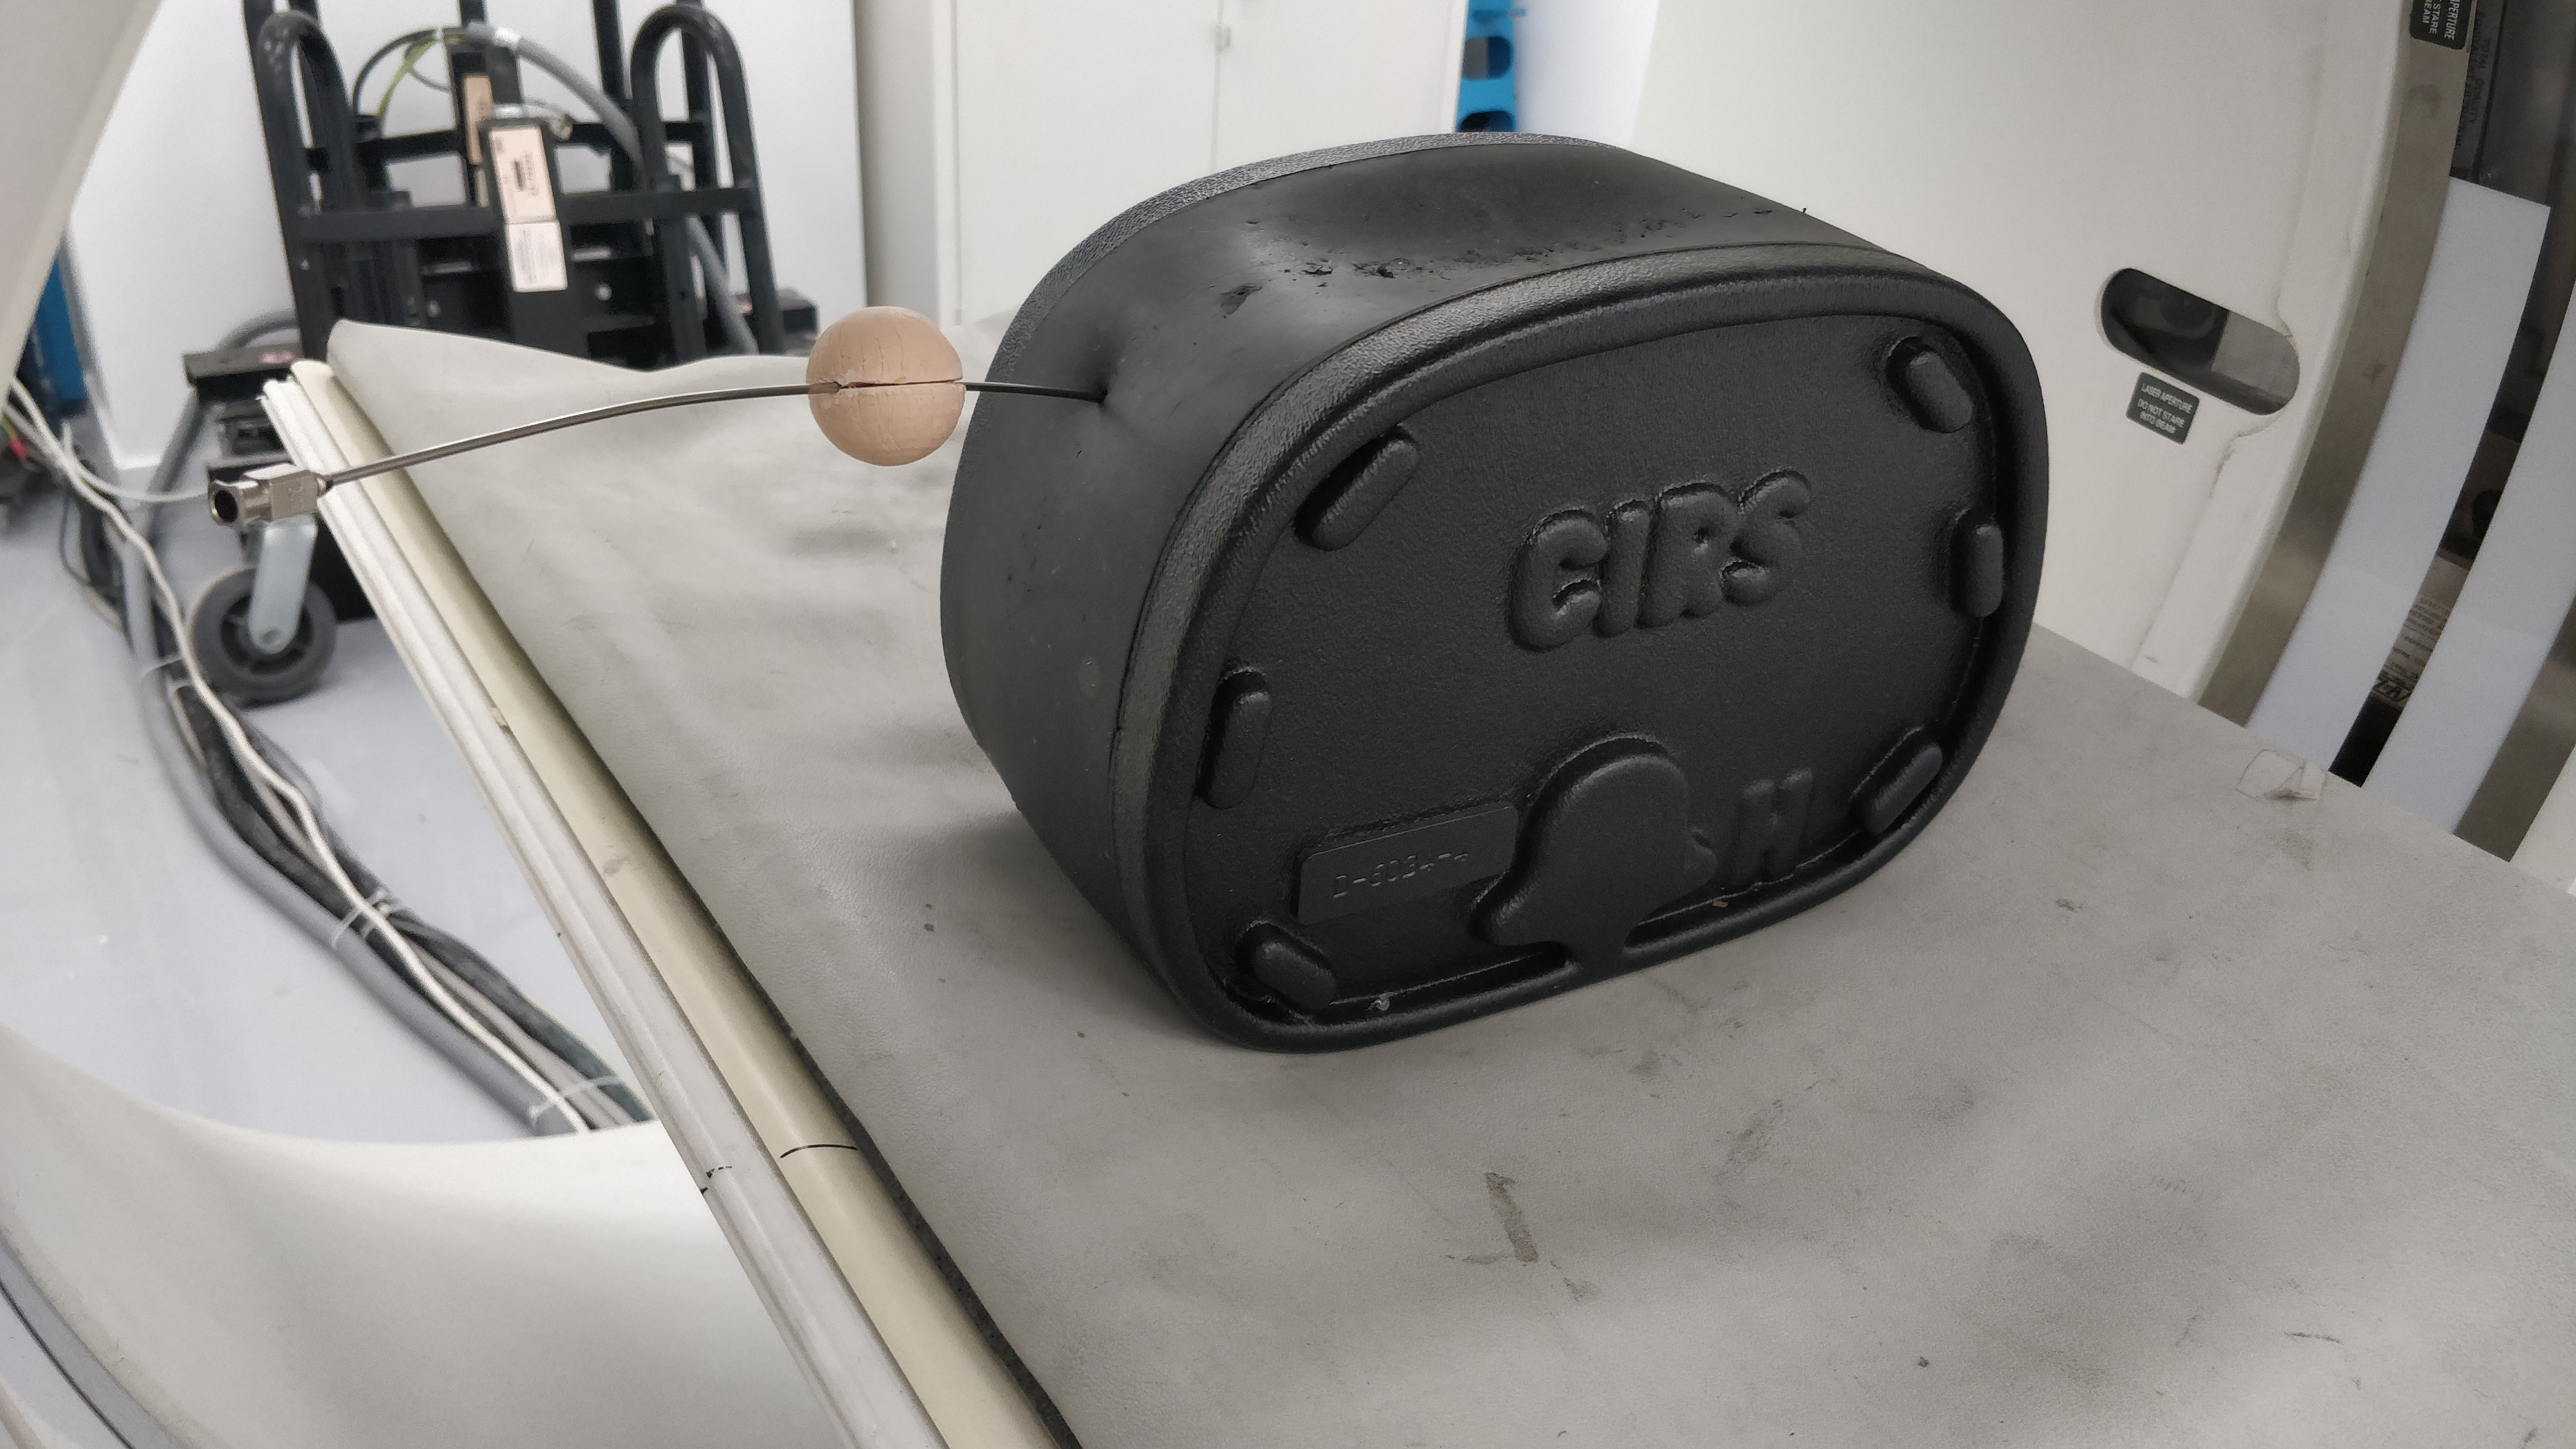
\includegraphics[width=8cm]{long_needle_phantom.jpg}
% \caption{\small{Photograph of the long flexible needle with spherical marker inserted into abdomen phantom lying on the CT scanner bed.}}
% \label{long_needle_fig}
% \end{figure}

% \begin{figure}[t]
% \centering
% 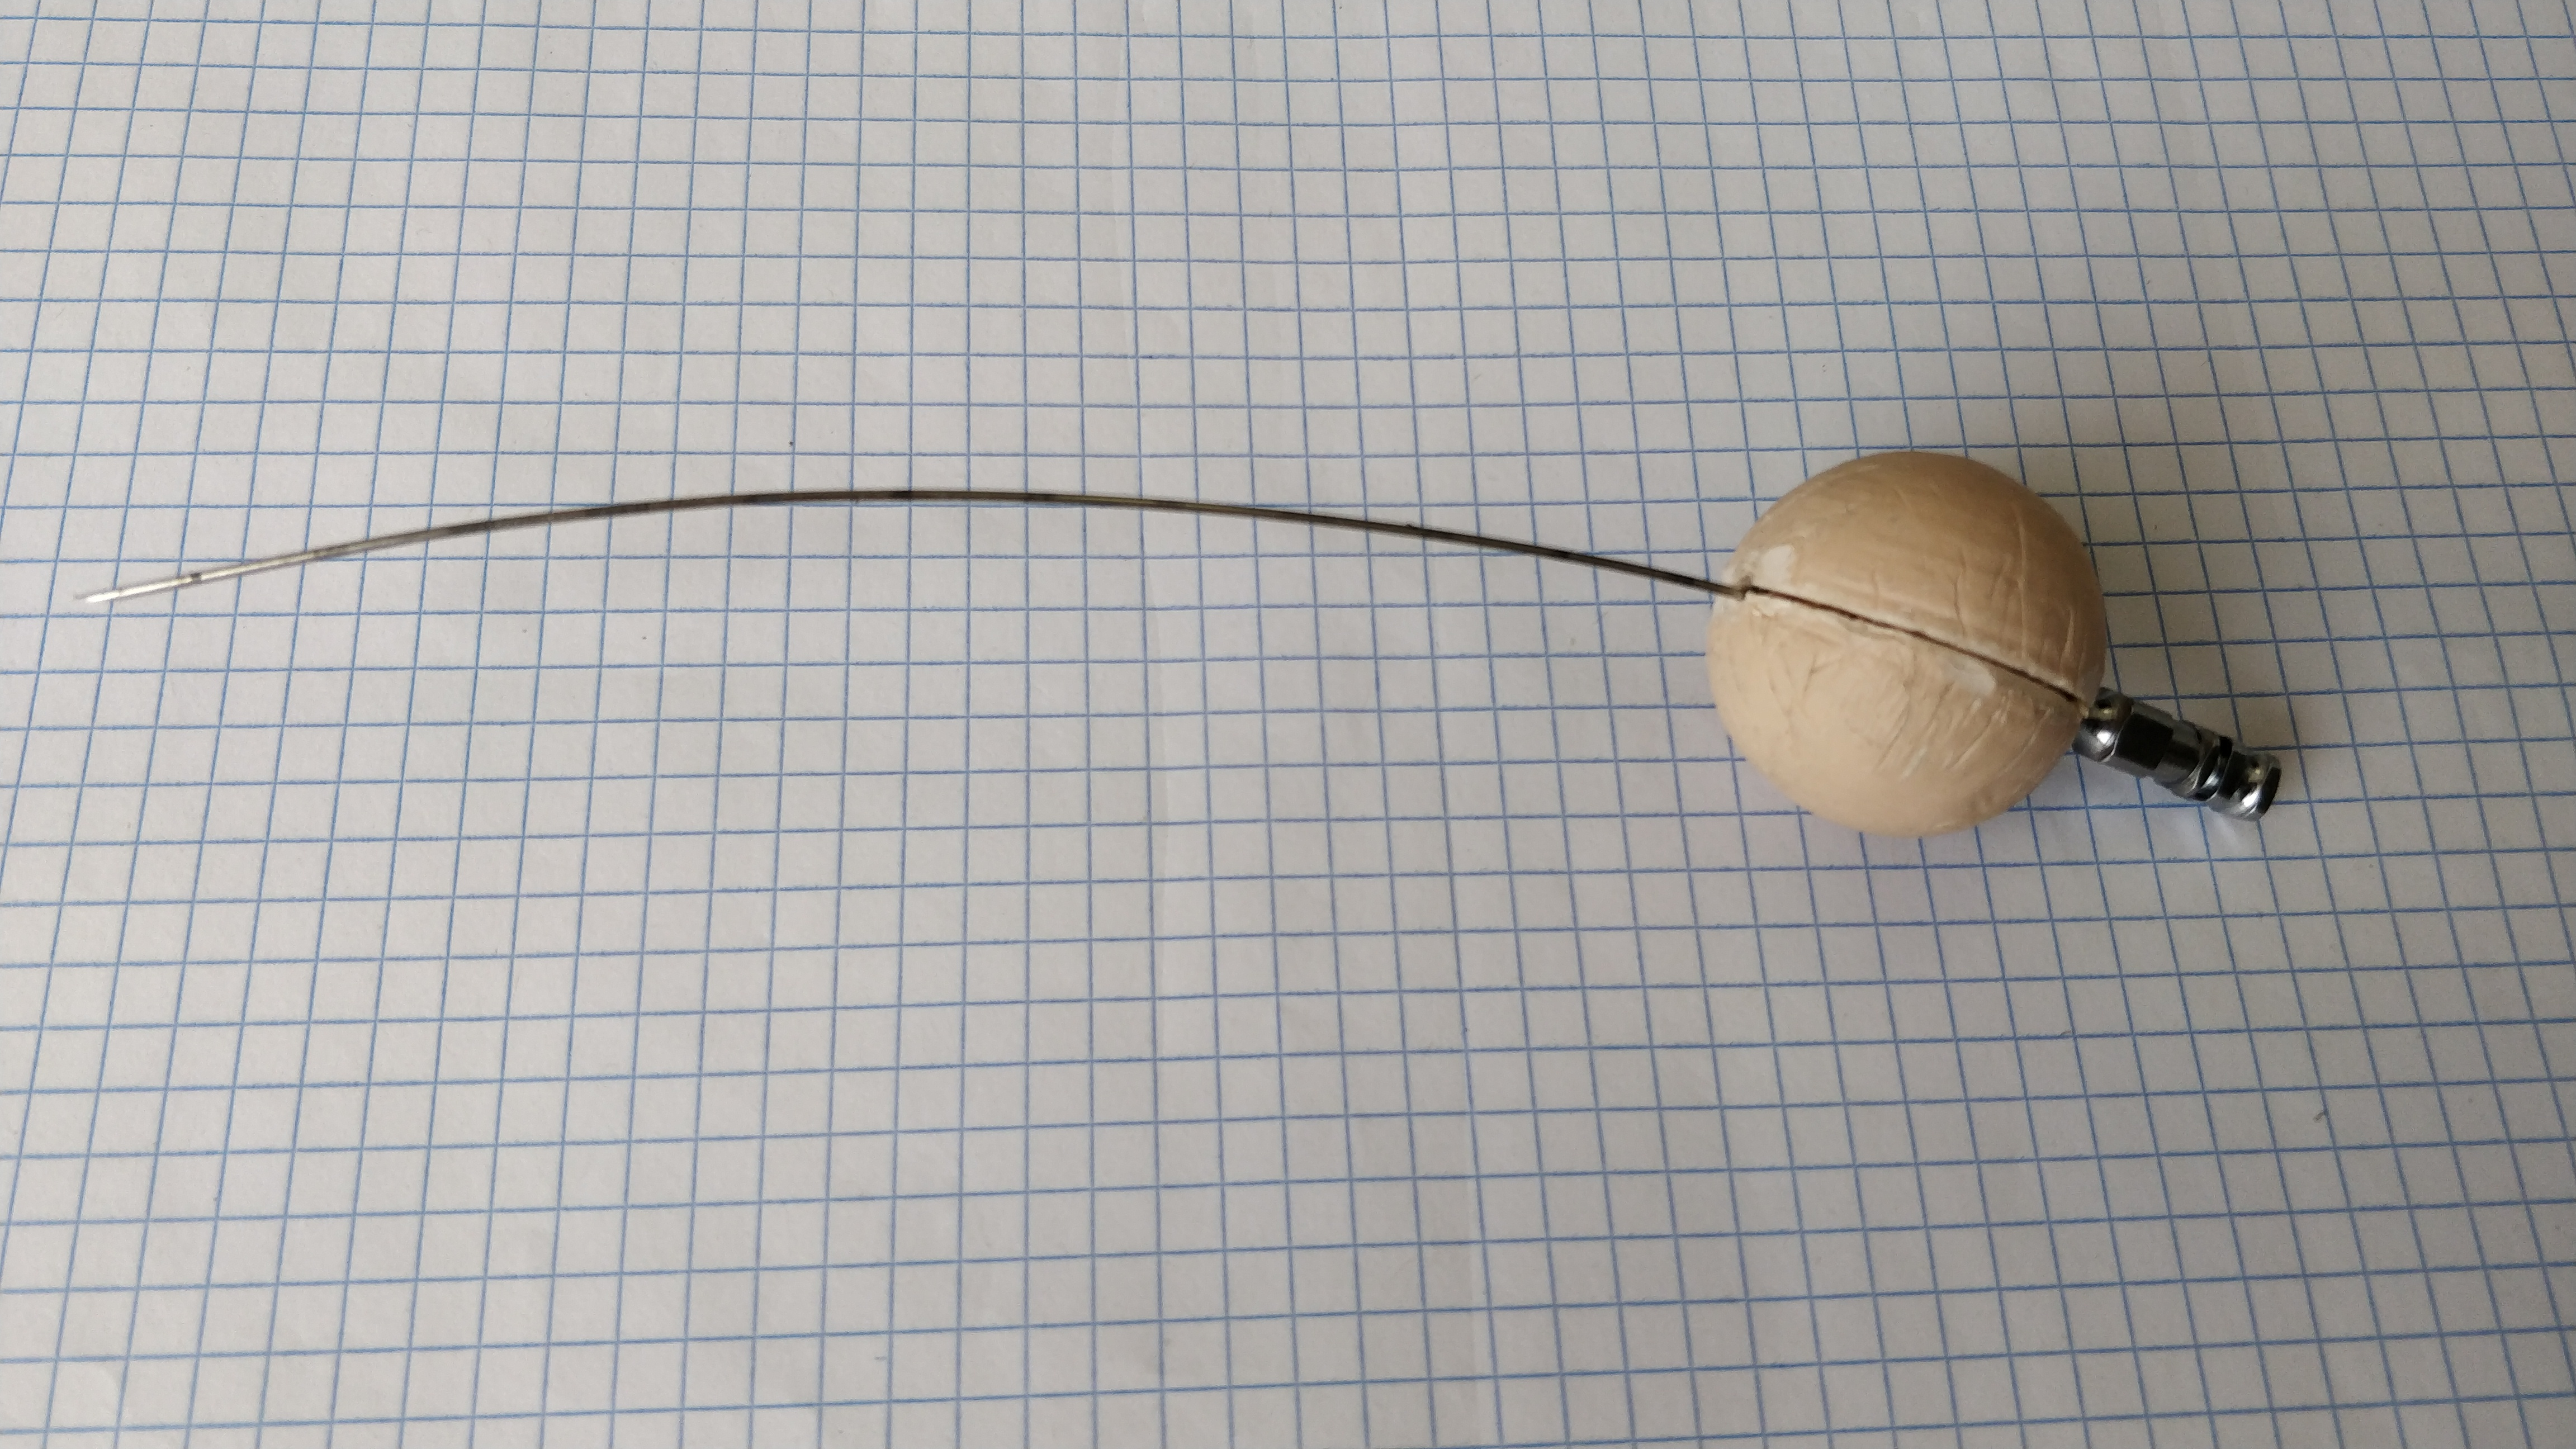
\includegraphics[width=8cm]{short_needle.jpg}
% \caption{\small{Photograph of the short flexible needle with spherical marker attached at 135mm from the tip.}}
% \label{short_needle_fig}
% \end{figure}


\begin{figure*}[t]
  \centering
  \subfloat[]{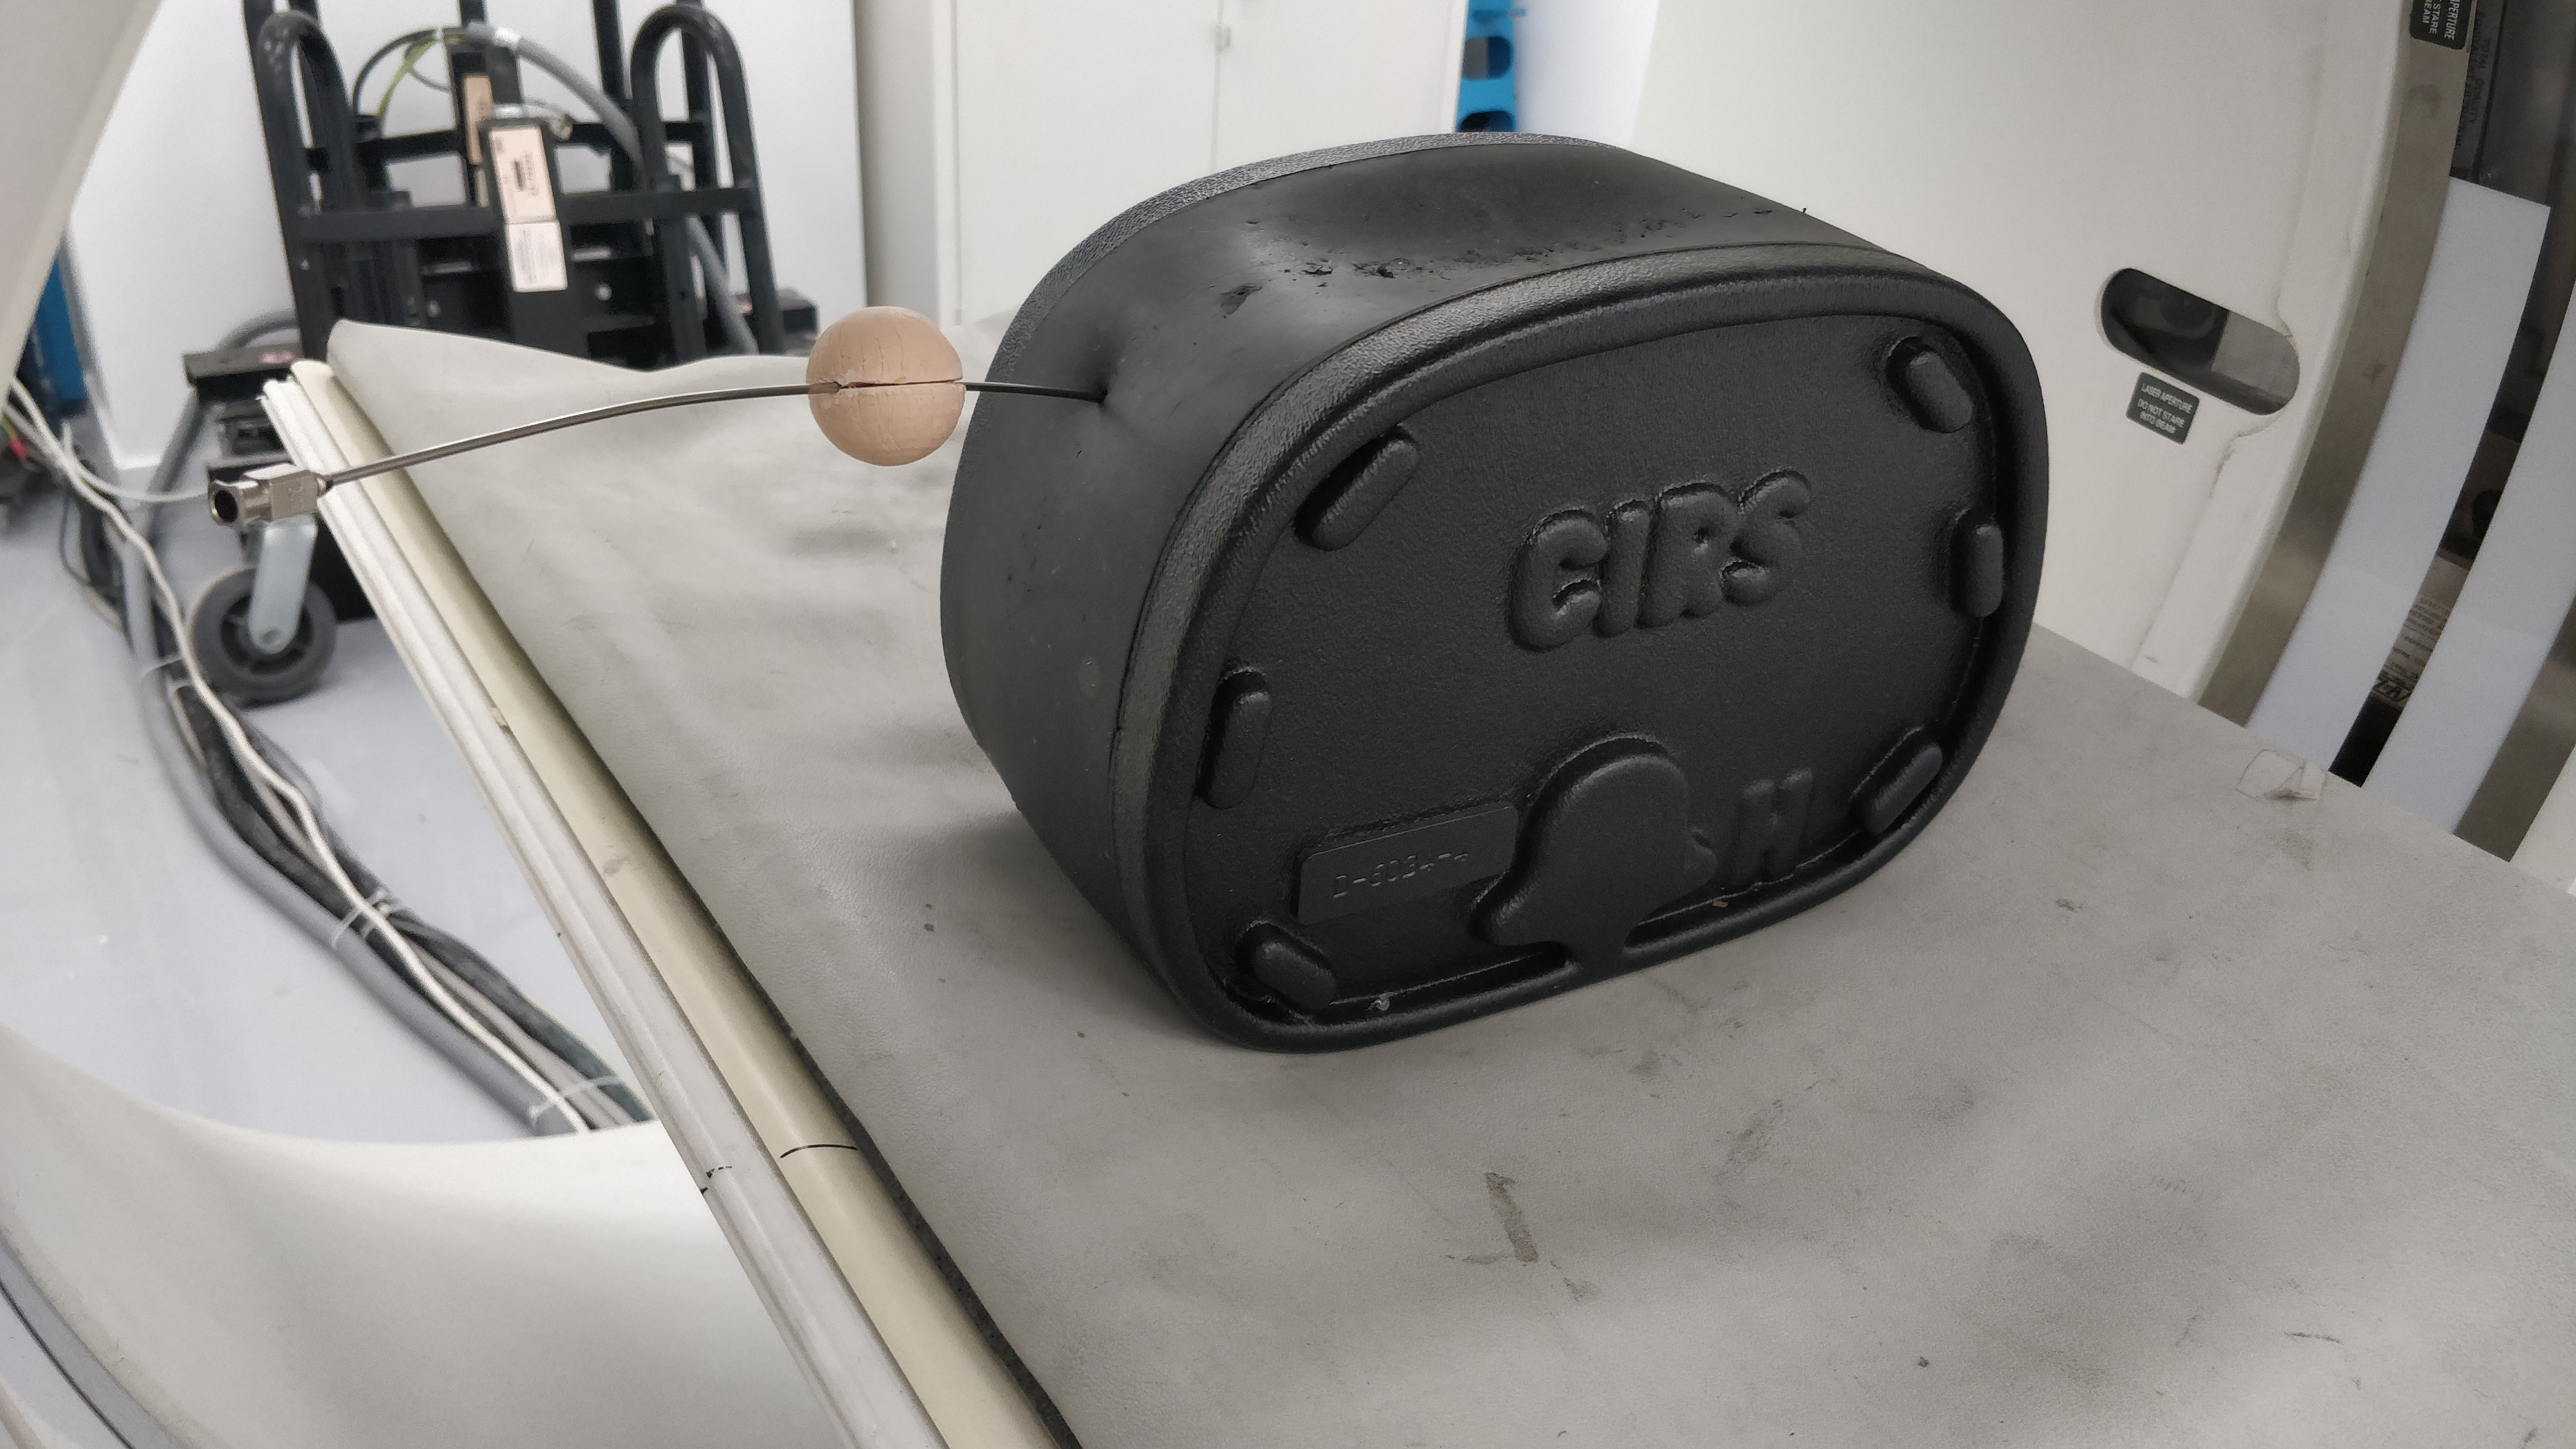
\includegraphics[width=0.45\textwidth]{long_needle_phantom.jpg}
  \label{long_needle_fig}}
  \hfill
  \subfloat[]{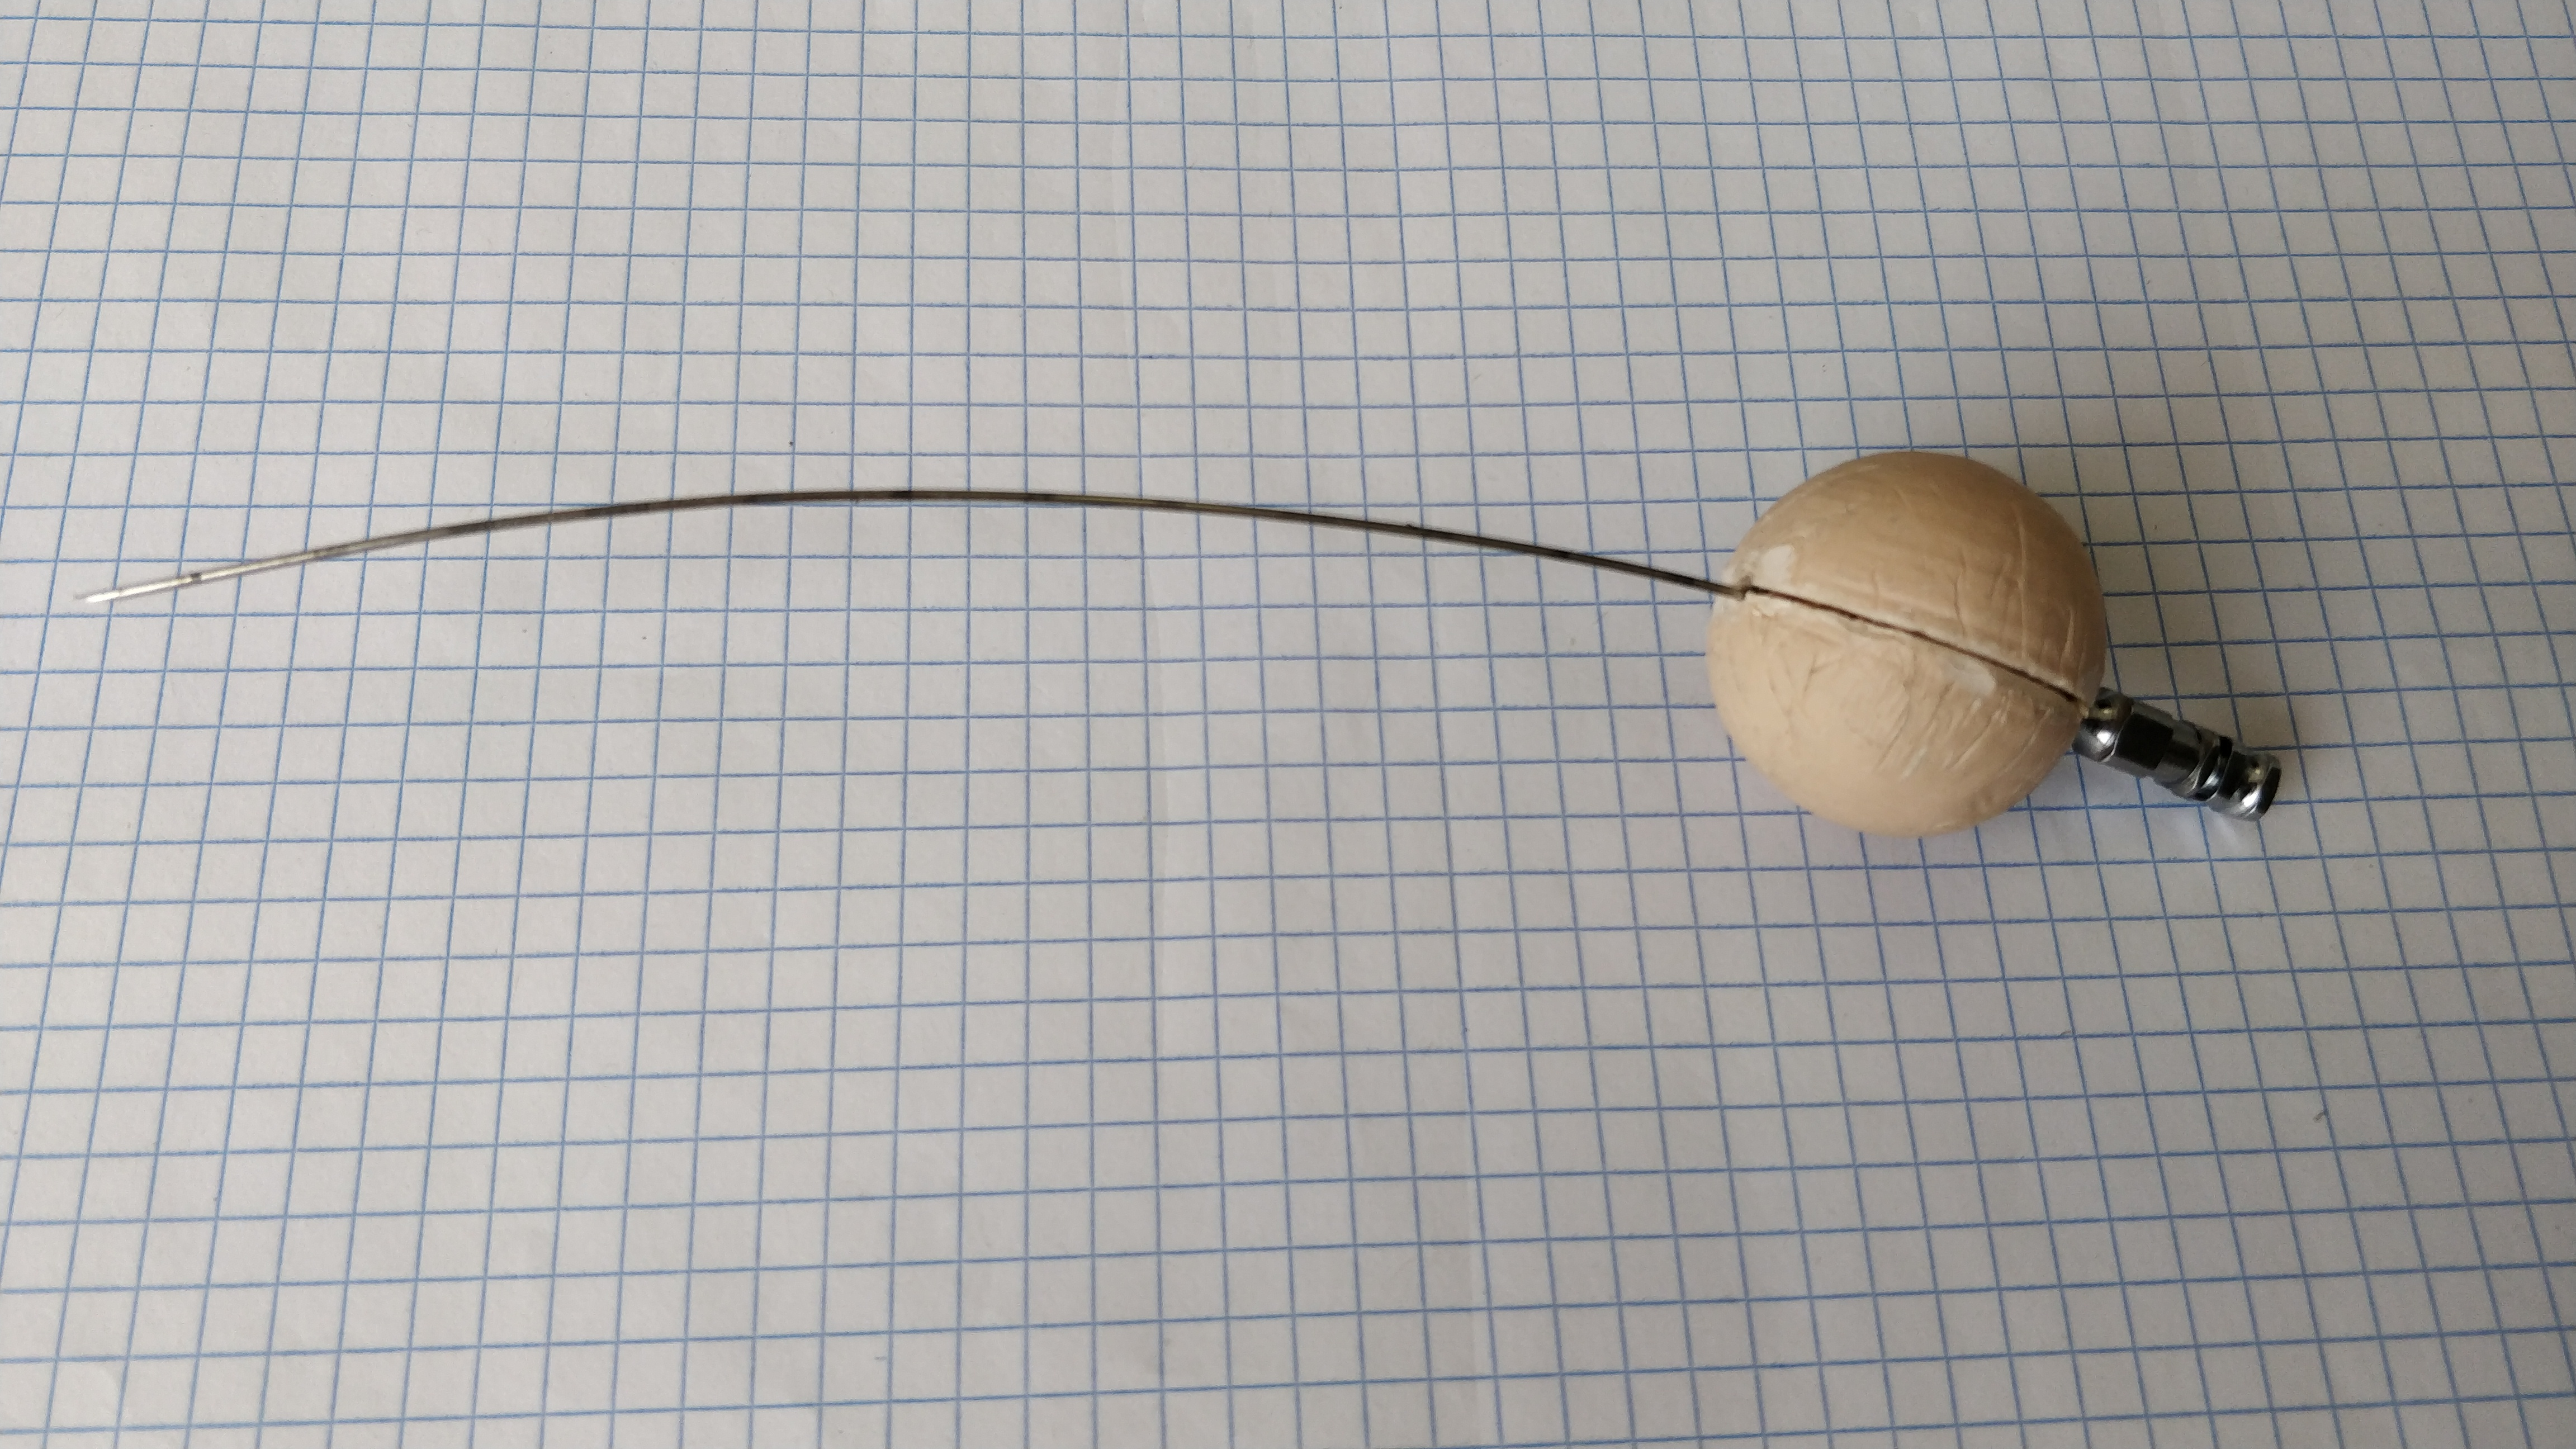
\includegraphics[width=0.45\textwidth]{short_needle.jpg}
  \label{short_needle_fig}}
  \caption{Experimental setup for flexible needle insertion in an abdomen phantom. (a) Photograph of the long flexible needle with a spherical marker affixed to it inserted into abdomen phantom on the CT scanner bed; (b) Photograph of the short flexible needle with the spherical marker affixed to it at 135mm from the tip.}
    \label{fig:figures/fractional}
\end{figure*}

\begin{table}[t]
\begin{center}
\begin{tabular}{|c||c|c|c|c|}
\hline
Scan & Reg. error & Marker & Tip error & Trajectory\\
ID  & [mm] & error [mm] & [mm] & error  [mm]\\
\hline
\hline
L1 & 1.4 & 1.9 & 2.6 & 0.7\\
\hline
L2 & 0.7 & 0.8 & 1.9 & 0.6\\
\hline
L3 & 0.6 & 0.3 & 4.3 & 0.9 \\
\hline
L4 & 1.0 & 0.8 & 2.0 & 0.5\\
\hline
S1 & 1.4 & 1.1 & 2.4 & 0.5\\
\hline
S2 & 1.2 & 1.5 & 1.4 & 0.6\\
\hline
S3 & 1.5 & 0.9 & 2.2 & 0.9\\
\hline
\hline
L & 
0.9 $\pm\hspace{0.04cm}$ 0.4 & 
1.0 $\pm\hspace{0.04cm}$ 0.7 & 
2.7 $\pm\hspace{0.04cm}$ 1.1 & 
0.7 $\pm\hspace{0.04cm}$ 0.2\\
\hline
S & 
1.4 $\pm\hspace{0.04cm}$ 0.2 &  
1.2 $\pm\hspace{0.04cm}$ 0.3 & 
2.0 $\pm\hspace{0.04cm}$ 0.5 &  
0.7 $\pm\hspace{0.04cm}$ 0.2\\
\hline
ALL & 
1.1 $\pm\hspace{0.04cm}$ 0.4 &  
1.0 $\pm\hspace{0.04cm}$ 0.5 &  
2.4 $\pm\hspace{0.04cm}$ 0.9 &  
0.7 $\pm\hspace{0.04cm}$ 0.2\\
\hline
\end{tabular}
\caption{\small{Summary of experimental results. L/S stands for long/short needle, respectively.
The bottom part of the table shows means and standard deviations across the long, short and all scans in the dataset.}}
\label{results_table}
\end{center}
\end{table}


\begin{figure}[t]
\centering
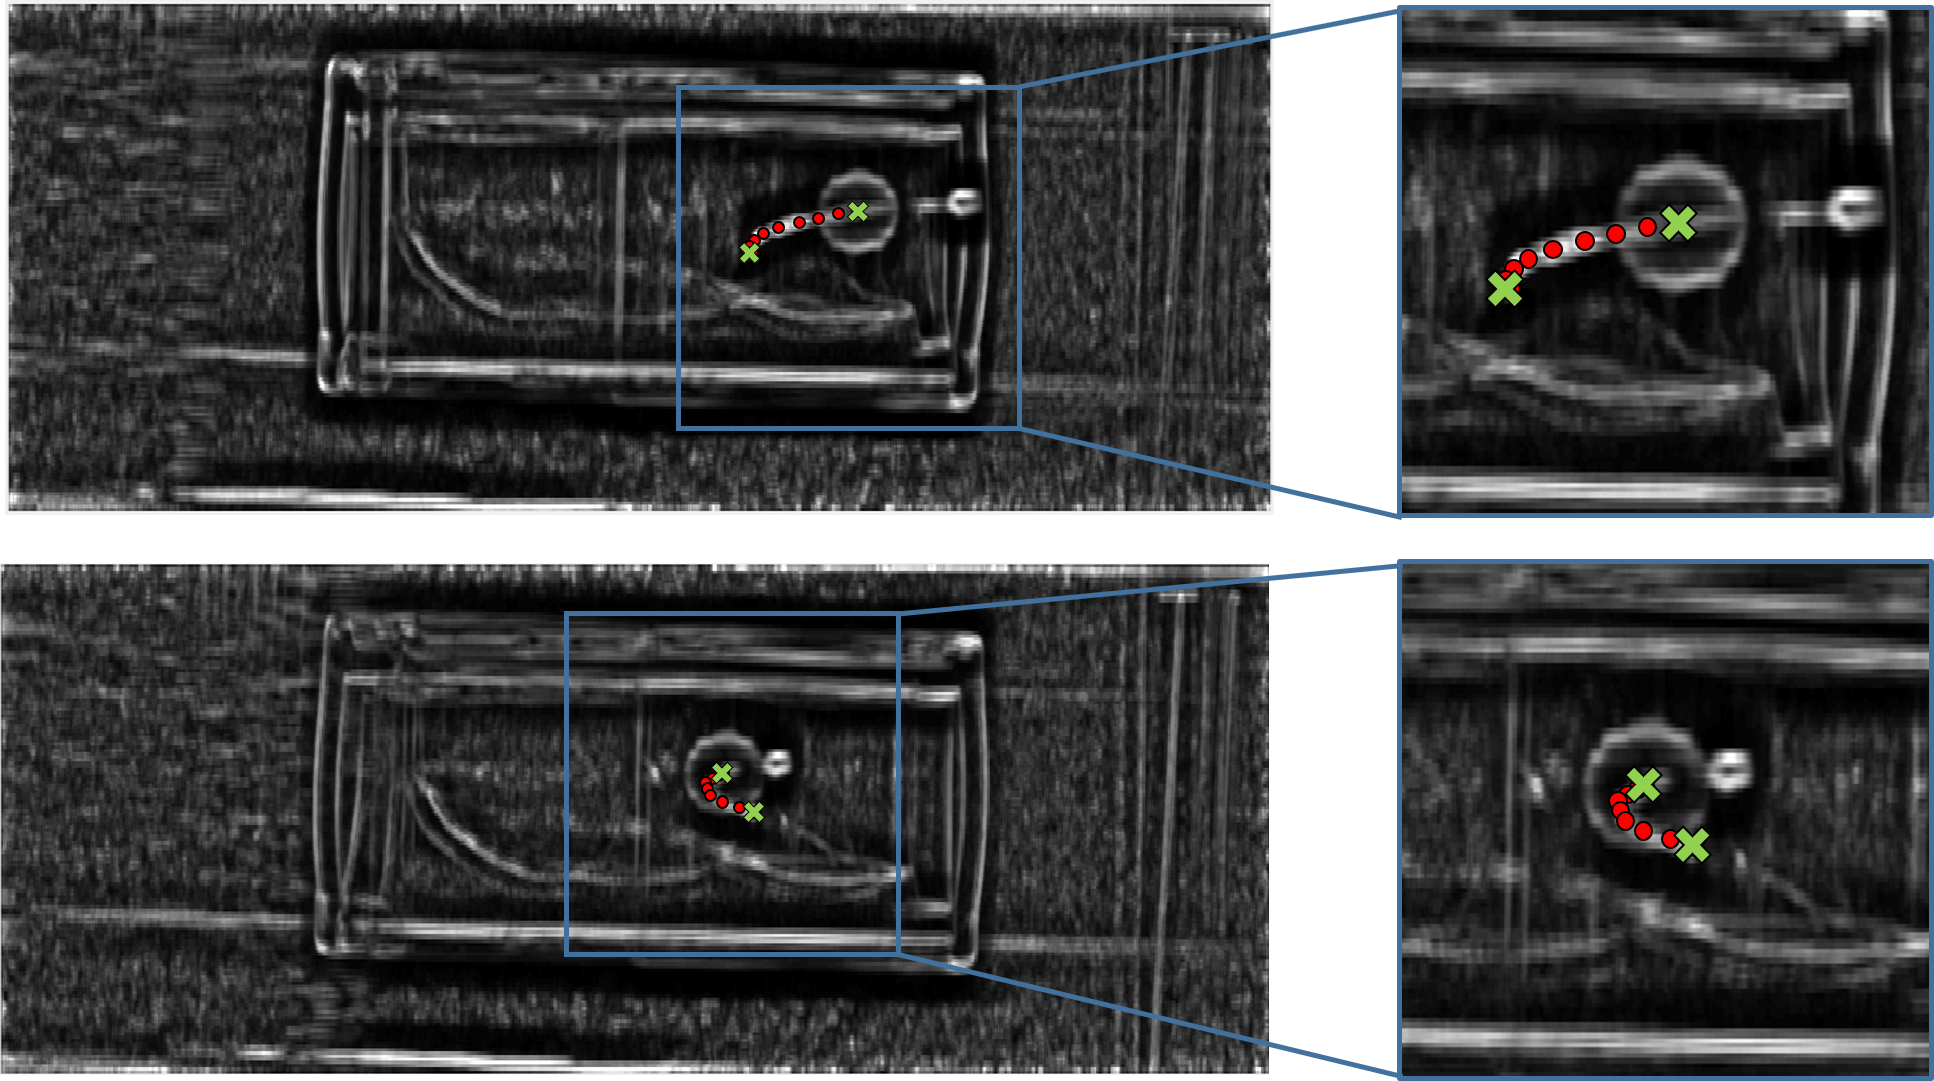
\includegraphics[width=\textwidth]{projection_diff_images.png}
\caption{Projection difference images for two views from one scan of the short flexible needle (left), and zoomed in on the needle in each image (right). The green crosses indicate the ground truth spherical marker center and the needle tip; the red dots indicate the landmark points computed by the incremental flexible needle trajectory algorithm.}
\label{proj_diff_fig}
\end{figure}

The full baseline scan was registered to each sparse scan with the flexible needle inserted using 3D Radon-space rigid registration. The registration accuracy was evaluated as the root-mean-square of differences between the voxels coordinates after rigid registration transformation and by image-space registration of the reconstructed images. A sparse set of 24 evenly spaced view angles in the range [0$^\circ$,180$^\circ$) was used for 3D Radon-space registration and flexible needle trajectory fitting as in the rigid needle experiments in \cite{medan2017reduced}. The choice of 24 view angles was selected from experiments with various values since it proved to be a good trade-off between robustness and potential dose reduction. The segment length parameter $\Gamma$ was set to 15mm. Experiments showed that lower values were not robust to feature noise in the optimization of segments directions, while greater values overshoot the typical bending of the needles in the experiments.

The spherical marker center ground truth coordinates was obtained by manual localization on the reconstructed images. The flexible needle trajectory ground truth was traced in 3D image space by manually placing landmark points on a volumetric difference image and then fitting them to a 3D cubic B\'ezier curve. The flexible needle tip ground truth location was defined as the point on the needle trace found at the known tip-marker distance. The flexible needle trajectory error was evaluated as the root-mean-squared distance of points along the fitted curve to the nearest point on the ground-truth B\'ezier curve.

Table \ref{results_table} summarizes the results of the flexible needle tip localization for seven CT scans: four with the long needle (L1-4) and three with the short needle (S1-3). One of the scans (L3) yields a large tip localization error due to the needle trajectory being very close to in-plane with the axial plane (Fig. \ref{multislices_fig}). In our method, long needle segments that are in-plane lead to inaccurate estimation of the trajectory since the projections of such segments appear as horizontal lines in the projection difference images regardless of the orientation within the plane \cite{medan2017reduced}. Thus, in-plane needle insertion should be avoided to enable the recovery of the needle orientation as an intersection of non-parallel planes.

The running time of our implementation is 200-250 seconds on an Intel i7 CPU running un-optimized Matlab code. To allow our method to be used in a clinical setting, the code should be optimized and paralelized for GPU computations so as to reduce the running time to 2-5 seconds. The parallelization is achieved in the projection difference computation step by computing the projection difference images in parallel and in the subsequent landmark point additions.  

\section*{Discussion}

\begin{figure*}[t]
\centering
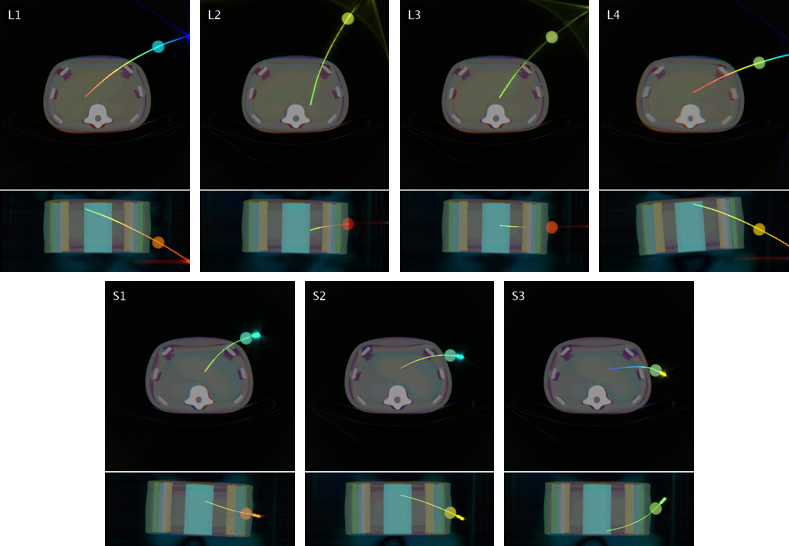
\includegraphics[width=\textwidth]{multislices.png}
\caption{Axial and coronal multi-slice views (top and bottom of each individual image, respectively) of the abdomen phantom with flexible needle (L - long needle, S - short needle) inserted in various positions. The multi-slice views are generated by assigning a color map to show the depth of each slice in the direction perpendicular to the image plane.}
\label{multislices_fig}
\end{figure*}

The key novelty of our method is the simultaneous tracking of a flexible needle and the registration of the patient location with respect to a baseline scan by fractional scanning, which precludes the reconstruction of the scanned image.  The computed flexible needle location can be displayed with respect to the baseline CT scan images in 2D or 3D to provide visual feedback to the clinician. The resulting augmented images are free of imaging artifacts and allow an unobstructed view of the target tissue and its surroundings. The accurate flexible needle location is of particular use for robotically driven needles to determine and adjust the needle insertion trajectory with substantially less radiation dose. 

Note that the spherical marker that is attached to the flexible needle is unobtrusive and does not add a burden to the intervention work flow since it only requires attaching a spherical marker to the flexible needle by the medical staff before the intervention. The potential ten-fold reduction in radiation dose is much more substantial than that of existing methods, i.e. about x2-3 of a full scan. 

{\em Method limitations}: our method is applicable to situations in which the patient anatomy baseline and repeat scans present minimal or no deformations and rigid registration can be used to align them. The scan field of view should include both the flexible needle and the spherical marker and should avoid in-plane needle insertion (an out-of-plane angle $>3^o$ suffices). 

{\em Study limitations:} the scope of our study is limited to several scans of an abdomen phantom. Fractional scanning is simulated from full scan data by omitting most of the repeat scan data used as input for the algorithm. To implement our method on a commercial CT scanner, fractional scanning can be achieved by fast modulation of the X-ray tube current and/or voltage, or by fast mechanical X-ray  collimation during scan acquisition. Fractional scanning can be realized by software (scanner controller), while collimation requires hardware development.  Both are beyond the scope of this work.
 
\section*{Conclusions}
We have presented a new method for flexible needle and patient localization in interventional CT procedures based on fractional CT scanning.
Our method accurately localizes the trajectory of a flexible needle to which a spherical marker is attached at a known distance from the tip with respect to a baseline scan of patient in the CT scanner coordinate frame. The computations are performed in 2D projection difference images computed from 3D Radon data in which the needle and the spherical marker appear as prominent features. 
The localization is achieved with a significantly lower dose compared to a full scan using sparse view angle sampling and without reconstructing the CT image of the repeat scan.

The main advantages of our method are:
1) accurate and robust localization of a flexible needle trajectory and its tip without image reconstruction;
2) significant dose reduction for each individual repeat scan localization;
3) simultaneous patient registration and flexible needle localization for every single scan; 
4) fully automatic method with no calibration and/or manual setup required; 
5) a simple and inexpensive spherical marker attached at a predefined distance to a flexible needle is required; 
6) artifact-free monitoring of the flexible needle tip and trajectory with respect to the baseline scan.

The novelties our method with respect to our previous paper are: 1) it accounts for needle bending during the insertion; 2) it tracks the entire needle, not only the tip; 3) it improves the accuracy and robustness of the spherical marker localization; 4) it validates the method in a new experimental setup that includes two types of needles. 

Our experimental results on an abdominal phantom study
in cooperation with a leading CT manufacturer yield a mean needle trajectory localization error of 0.7 $\pm$ 0.2mm and a mean tip localization error of 2.4 $\pm$ 0.9 mm, an accuracy comparable to other 3D imaging methods. The significant dose reduction of x7.5-10 with respect to a full scan enables more frequent needle trajectory localization during the needle insertion for a similar total dose, or a reduced total dose for the same localization frequency.

Our current work aims at developing sparse repeat scanning methods for Region-Of-Interest reconstruction and  for deformable registration with a general low-order parametric
model in 3D Radon space and without reconstructing the repeat \cite{adelmanmsc2018}. These methods may help account for anatomy deformations caused by breathing and other sources. 

\bibliographystyle{spbasic_order_of_appearance}
\bibliography{flexible_needle}

\end{document}
% end of file template.tex

